\documentclass{article}%ctex
\input{~/code/math_commands.tex}

\usepackage{graphicx}
\usepackage{tikz}


\title{\huge Lecture 4 From Directed to Undirected Graphical Models\\
\normalsize}
\author{Xuanxi Zhang}
\begin{document}
\maketitle


\section*{Topics:}
\begin{itemize}
    \item Gibbs distributions / Markov Models
    \item Existence and Uniqueness of Markov Models
    \item Directed vs Undirected Graphical Models
\end{itemize}

\paragraph{Recall from Lecture 3: Bayesian Nets / Directed Graphical Models}
\[
P(X_1, X_d) = \prod_i P(X_i \mid X_{A(i)})
\]

\textbf{Pros:}
\begin{itemize}
    \item \textbf{Efficient:} Generative process along topological order.
    \item \textbf{Self-normalised:} Local factors are probabilities, so the joint model is automatically normalised.
\end{itemize}

\textbf{Cons:}
\begin{itemize}
    \item Conditional independencies are not explicit (rely on d-separation!).
    \item Lack of existence \& uniqueness.
\end{itemize}

\textbf{
Can we alleviate some of these issues?}

\section{Undirected Graph Representation}

Consider a graph \( G = (V, E) \) with \( V = \{X_1, \dots, X_n\} \) (random variables) and  \( E \) (undirected edges)

\begin{itemize}
    \item In the directed case, we first build a factorization of the joint probability, i.e., 
    \[
    P(X_1, \dots, X_n) = \prod_i P(X_i \mid X_{A(i)})
    \]
    Then, we ``draw'' an edge \( j \to i \) whenever \( j \in A(i) \).
    \item In the undirected case, first, we postulate that:
    \[
    X \perp Y \mid Z
    \]
    whenever nodes in \( Z \) separate (topologically) node \( X \) from \( Y \) on \( G \). This represents the \textbf{Markov property} on \( G \).
    
\end{itemize}

Conceptual Relationship
\begin{itemize}
    \item Undirected Graphical Models starts with a \textbf{Conditional Independence} to define the graph, then obain the \textbf{Factorization} from the graph.
    \item Directed Graphical Models starts with a \textbf{Factorization} to define the graph, then obtain the \textbf{Conditional Independence} from the graph.
\end{itemize}

\paragraph{Question:}
Are directed and undirected graphical models expressing the same \textbf{class of distributions}?

\textbf{NO!}

\paragraph{Example 1:}Given Conditional Independencies
\[
A \perp D \mid \{B, C\}
\]
\[
B \perp C \mid \{A, D\}
\] 
\begin{center}
    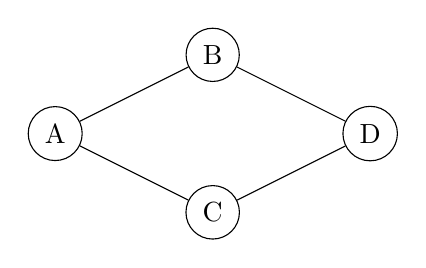
\begin{tikzpicture}
        \node (A) at (0,2) [circle,draw] {A};
        \node (B) at (2,3) [circle,draw] {B};
        \node (C) at (2,1) [circle,draw] {C};
        \node (D) at (4,2) [circle,draw] {D};
        
        \draw (A) -- (B);
        \draw (B) -- (D);
        \draw (A) -- (C);
        \draw (C) -- (D);
    \end{tikzpicture}
\end{center}
Can we build a directed graphical model consistent with these conditional independencies?


\paragraph{Example 2:} Given 
\begin{enumerate}
    \item \( X \perp Y \)
    \item \( X \not\perp Y \mid Z \)
\end{enumerate}
\begin{center}
    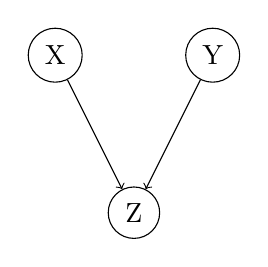
\begin{tikzpicture}
        \node (X) at (0,2) [circle,draw] {X};
        \node (Y) at (2,2) [circle,draw] {Y};
        \node (Z) at (1,0) [circle,draw] {Z};
        
        \draw[->] (X) -- (Z);
        \draw[->] (Y) -- (Z);
    \end{tikzpicture}
\end{center}

\textbf{Issue:} Constructing a undirected model leads to failures:
\begin{itemize}
    \item If \( X - Z - Y \), then (2) fails!
    \item If full connected, then (1) fails!
\end{itemize}

\paragraph{Conclusion:} Bayesian Nets (Directed Graphical Models) and Graphical Models (Undirected Graphical Models) have intersection but \textbf{not} equivalent!
\begin{itemize}
    \item BN: Models with ``canonical'' topological order.
    \item GM: Models with some \textit{exchangeability}.
\end{itemize}

\section{Parameterization of GM and Gibbs Distributions}

Recall BN Factorization:
\[
P(X_1, \dots, X_n) = \prod_i P(X_i \mid X_{A(i)})
\]
``Building blocks'' are \textbf{conditional probabilities}. This form compatible with topological order; however, \textbf{undirected models aim to remove this constraint}.

We still want a \textbf{local factorization} of the joint density (in order to beat the curse of dimensionality (CoD)). Let start with following formulation:
\[
P(X_1, \dots, X_n) = \prod_{C \in \mathcal{C}} \psi_C (X_C),
\]
where $\gC \subseteq \gP(\{1,2,\cdots,n\})$ to be determined. 
\(
X_C = \{X_i \mid i \in C\}
\) and $\psi_C$ is a potential function locally on $X_C$ (usually not a probability distribution).

We want this factorization to be compatible with the \textbf{Markov property} on \( G \), which means \( X_i \) and \( X_j \) are conditionally independent given the rest if \( i, j \) are not neighbors in the graph, which means
\[
    P \left( X_i, X_j \mid \{X_k\}_{k \neq i,j} \right) = F(X_i) G(X_j)
\]
Some calculation
\begin{align*}
P \left( X_i, X_j \mid \{X_k\}_{k \neq i,j} \right) =&\frac{P(X_1, \dots, X_n)}{\int P(X_1, \dots, X_n) \, dX_i \, dX_j}=\frac{\prod_{C \in \mathcal{G}} \psi_C (X_C)}
{\int \prod_{C \in \mathcal{G}} \psi_C (X_C) \, dX_i \, dX_j}
\end{align*}
Expanding the terms,
\[\prod_{C \in \mathcal{G}} \psi_C (X_C)=
\prod_{(i,j) \in C} \psi_C (X_C) \cdot 
\prod_{j \in C, i \notin C} \psi_C (X_C) \cdot 
\prod_{i \in C, j \notin C} \psi_C (X_C) \cdot
\prod_{i \notin C, j \notin C} \psi_C (X_C)
\]
Taking the integral leads to 
\[
P \left( X_i, X_j \mid \{X_k\}_{k \neq i,j} \right)=\frac{\prod_{(i,j) \in C} \psi_C (X_C)}{\int \prod_{(i,j) \in C} \psi_C (X_C) dX_i dX_j}\cdot\frac{\prod_{j \in C, i \notin C} \psi_C (X_C)}{\int \prod_{j \in C, i \notin C} \psi_C (X_C)dX_j} \cdot\frac{\prod_{i \in C, j \notin C} \psi_C (X_C)}{\int\prod_{i \in C, j \notin C} \psi_C (X_C) dX_i} 
\]

We want this function to be of the form:
\(
F(X_i) \cdot G(X_j)
\)

\begin{itemize}

\item $\Rightarrow$ \( (i,j) \) \textbf{cannot belong to any} \( C \)

\item $\Rightarrow$ $C$ only contains nodes $X_i$ that are connected with each other.

\item $\Rightarrow$ $\gC$ only contains \textbf{cliques} (fully connected subgraph) of \( G \).

    \item Since a clique \( C \) contains all smaller cliques \( C' \subset C \), we can reduce ourselves to the set \( \mathcal{G} \) of \textbf{maximal cliques}.
    \item \( C \) is a \textbf{maximal clique} if \( C \cup \{ x_i \} \) is not a clique for all \( i \notin C \).
\end{itemize}

\subsection{Summary}
\[
\mathcal{C} = \{ C \mid C \text{ is a maximal clique of } G \}
\]
\[
\psi_C(X_C) \text{ is an arbitrary non-negative potential.}
\]
Probability distribution is parameterized as 
\[
p(x) = \frac{1}{Z} \prod_{C \in \mathcal{C}} \psi_C (X_C),
\]
where the partition function is:
\[
Z = \int \left( \prod_C \psi_C (X_C) \right) dx.
\]

We say that \( P \) is a \textbf{Gibbs distribution} that factorizes over \( G \).

\subsection{Meaning of the local potentials}

\textbf{Example:}

\begin{center}
    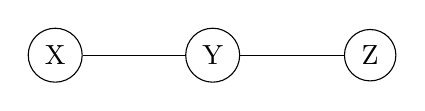
\begin{tikzpicture}
        \node (X) at (0,1) [circle,draw] {X};
        \node (Y) at (2,1) [circle,draw] {Y};
        \node (Z) at (4,1) [circle,draw] {Z};

        \draw (X) -- (Y);
        \draw (Y) -- (Z);
    \end{tikzpicture}
\end{center}

Given the independence:

\[
X \perp Z \mid Y
\]

we can factorize:

\[
P(X, Y, Z) = P(X \mid Y) P(Y) P(Z \mid Y)
\]

Rewriting,

\[
P(X, Y, Z) = P(X\mid Y) P(Y)^\alpha P(Y)^{1-\alpha} P(Z \mid Y)
\]

which gives us:

\[
\psi_1 (X,Y), \quad \psi_2 (Y,Z)
\]

where \( \psi_1, \psi_2 \) are \textbf{not} probability distributions.

\textbf{General Case:} 

\[
P(X, Y, Z) \neq P(X, Y) P(Y, Z).
\]

\section{From Graph to Markov Property}
We start form this question: given a graph \( G \), can we list all conditional independencies invovling a given point $X$?

\begin{definition}[Markov Blanket]
A set \( A \subseteq \mathcal{X} \) is a \textbf{Markov Blanket} for \( X \) if \( X \not\in A \), and \( A \) is a minimal set such that:
\[
X \perp \gX \setminus A \cup \{X\} \mid A.
\]
\end{definition}

The \textbf{Markov Blanket} in \textbf{undirected graphical models} is precisely the set of neighbors in \( G \)! Consider following example:
\begin{center}
    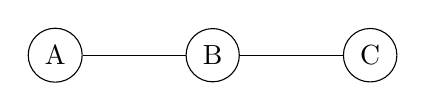
\begin{tikzpicture}
        \node (A) at (0,1) [circle,draw] {A};
        \node (B) at (2,1) [circle,draw] {B};
        \node (C) at (4,1) [circle,draw] {C};

        \draw (A) -- (B);
        \draw (B) -- (C);
    \end{tikzpicture}
\end{center}
with Gibbs Model
\[
P(a,b,c) = \frac{1}{Z} \psi_1(a,b) \cdot \psi_2(b,c)
\]
Lets verifying the markov Pproperty \( A \perp C \mid B \).
\begin{align*}
P(a,c \mid b) &= \frac{P(a,b,c)}{P(b)} = \frac{\psi_1(a,b) \cdot \psi_2(b,c)}{Z \cdot P(b)}= \frac{\psi_1(a,b) \cdot \psi_2(b,c)}{\int \psi_1(a,b) \cdot \psi_2(b,c) \, da \, dc}= \frac{\psi_1(a,b)}{\int \psi_1(a,b) \, da} \cdot \frac{\psi_2(b,c)}{\int \psi_2(b,c) \, dc}
\end{align*}


This is an instance of a more general property:

\begin{theorem}[ K \& F, \text{Theorem 4.1} ]
    If \( P \) is a \textbf{Gibbs distribution} factorizing over \( G \), then \( G \) is an \(\mathcal{I}\)-map for \( P \), i.e.,
\[
\mathcal{I}(G) \subseteq \mathcal{I}(P)
\]
\end{theorem}

\textbf{Proof Sketch}
If \( Y \) separates \( X \) and \( Z \), then there are no direct edges between \( X \) and \( Z \). Any clique is either in \( X \cup Y \) or in \( Z \cup Y \).
Thus,
\[
P(X_1, \dots, X_n) = \frac{1}{Z} \psi_1(X,Y) \cdot \psi_2(Z,Y)
\]

which reduces to the \textbf{previous example}. \(\square\)

\section{From Markov Property to Graph}
In last section, we showed that given a graph \( G \)(and corresponding gibbs distribution), we can deduce the Markov property. Can we deduce that \( P \) is Gibbs w.r.t \( G \) just from the Markov property?

\begin{theorem}[Hammersley-Clifford]
Let \( P > 0 \) over \( X \), and let \( G \) be an \textbf{undirected graph} over \( X \). If \( G \) is an \(\mathcal{I}\)-map over \( P \), then \( P \) is a \textbf{Gibbs distribution} w.r.t. \( G \).
\end{theorem}
\textbf{Proof: }Recitation

\textbf{Interpretation:} The Hammersley-Clifford theorem gives us an \textbf{equivalence} between two sources of structure:
\begin{itemize}
    \item \textbf{Factorization} (expressed at the level of the density)
    \[
    P(X_1, \dots, X_n) = \frac{1}{Z} \prod_C \psi_C (X_C)
    \]
    (Gibbs Distribution)
    \item \textbf{Independence} (expressed at the level of random variables)
    \[
    X_i \perp X_j \mid X_{k}, k \notin \{i,j\}
    \]
    (Markov Assumption)
\end{itemize}

Remark: Positivity assumption is necessary! (We'll see a counter-example in HW 2.)












\end{document}